\chapter{Bipolar Junction Transistor-Solutions}
\begin{enumerate}
	\item The transistor in the given circuit has $h_{f e}=35 \Omega$ and $h_{i e}=1000 \Omega$. If the load resistance $R_{L}=1000 \Omega$, the voltage and current gain are, respectively.
{	\exyear{NET/JRF(JUNE-2012)}}
\begin{tasks}(1)
	\task[\textbf{A.}] $-35$ and $+35$
	\task[\textbf{B.}] 35 and $-35$
	\task[\textbf{C.}] 35 and $-0.97$
	\task[\textbf{D.}]  $0.98$ and - 35
\end{tasks}
\begin{figure}[H]
	\centering
	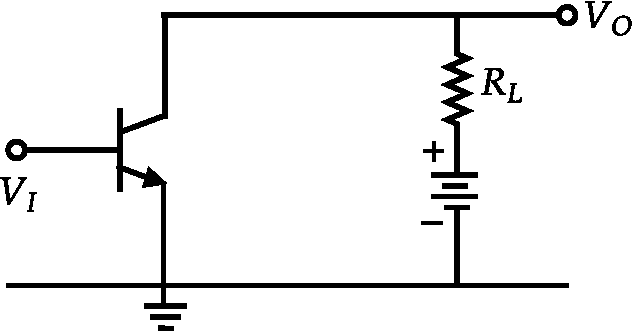
\includegraphics[height=3cm,width=5cm]{e-10}
\end{figure}
\begin{answer}
So the correct answer is \textbf{Option (A)}
\end{answer}
	\item A silicon transistor with built-in voltage $0.7 \mathrm{~V}$ is used in the circuit shown, with $V_{B B}=9.7 V, R_{B}=300 k \Omega, V_{C C}=12 V$ and $R_{C}=2 k \Omega$. Which of the following figures correctly represents the load line and quiescent $Q$ point?
{	\exyear{NET/JRF(JUNE-2013)}}
\begin{figure}[H]
\centering
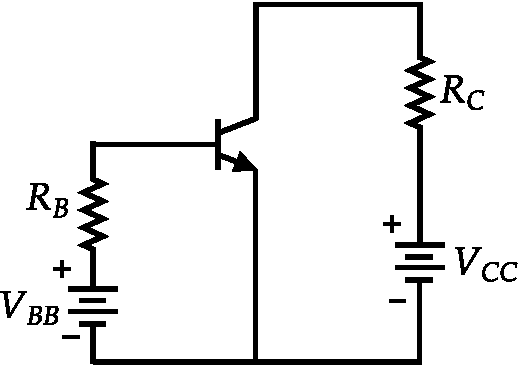
\includegraphics[height=3.5cm,width=5cm]{e-17}
\end{figure}
\begin{tasks}(2)
\task[\textbf{A.}] \begin{figure}[H]
	\centering
	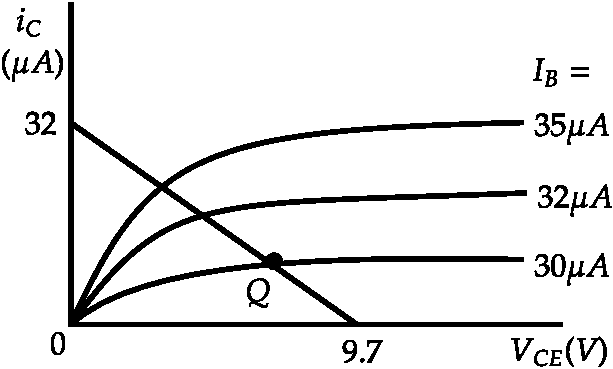
\includegraphics[height=3.3cm,width=5.5cm]{e-17a}
\end{figure}
\task[\textbf{B.}] \begin{figure}[H]
	\centering
	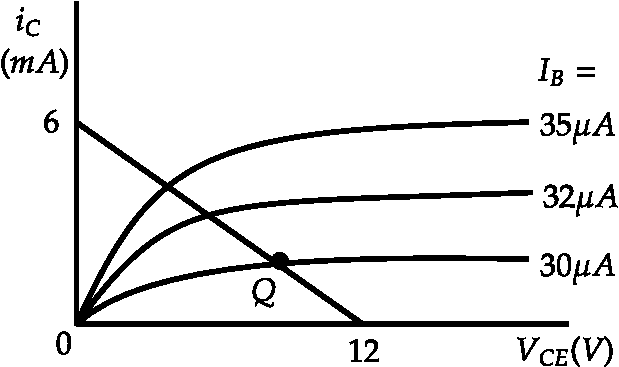
\includegraphics[height=3.3cm,width=5.5cm]{e-17b}
\end{figure}
\task[\textbf{C.}] \begin{figure}[H]
	\centering
	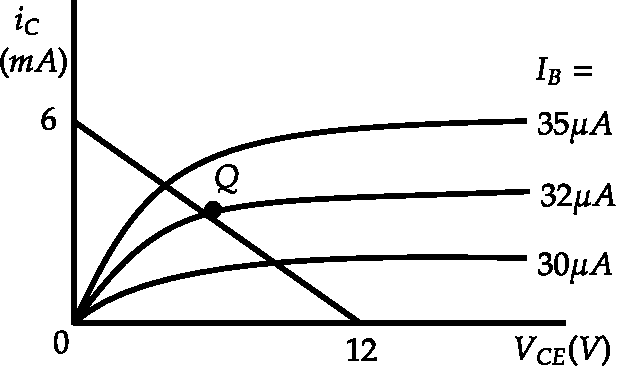
\includegraphics[height=3.3cm,width=5.5cm]{e-17c}
\end{figure}
\task[\textbf{D.}] \begin{figure}[H]
	\centering
	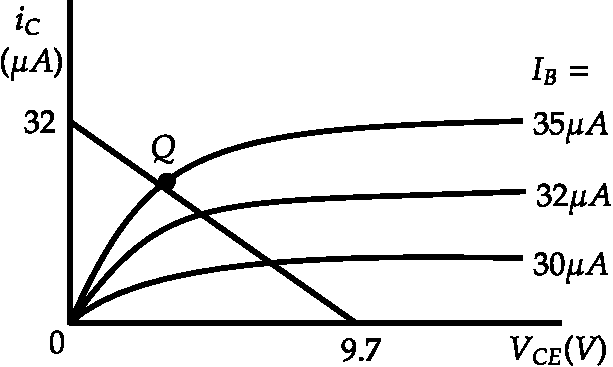
\includegraphics[height=3.3cm,width=5.5cm]{e-17d}
\end{figure}
\end{tasks}
\begin{answer}
\begin{align*}
I_{B}&=\frac{V_{B B}-V_{B E}}{R_{B}}=\frac{9.7-0.7}{300 \times 10^{3}}=30 \mu A\\\text{ and } I_{C, s a t}&=\frac{V_{C C}}{R_{C}}=\frac{12}{2 \times 10^{3}}=6 m A
\end{align*}
So the correct answer is \textbf{Option (B)}
\end{answer}
	\item The input to a lock-in amplifier has the form $V_{i}(t)=V_{i} \sin \left(\omega t+\theta_{i}\right)$ where $V_{i}, \omega, \theta_{i}$ are the amplitude, frequency and phase of the input signal respectively. This signal is multiplied by a reference signal of the same frequency $\omega$, amplitude $V_{r}$ and phase $\theta_{r}$. If the multiplied signal is fed to a low pass filter of cut-off frequency $\omega$, then the final output signal is
{	\exyear{NET/JRF(JUNE-2013)}}
\begin{tasks}(2)
\task[\textbf{A.}] $\frac{1}{2} V_{i} V_{r} \cos \left(\theta_{i}-\theta_{r}\right)$
\task[\textbf{B.}] $V_{i} V_{r}\left[\cos \left(\theta_{i}-\theta_{r}\right)-\cos \left(\frac{1}{2} \omega t+\theta_{i}+\theta_{r}\right)\right]$
\task[\textbf{C.}] $V_{i} V_{r} \sin \left(\theta_{i}-\theta_{r}\right)$
\task[\textbf{D.}] $V_{i} V_{r}\left[\cos \left(\theta_{i}-\theta_{r}\right)+\cos \left(\frac{1}{2} \omega t+\theta_{i}+\theta_{r}\right)\right]$
\end{tasks}
\begin{answer}
\begin{align*}
V&=V_{r} \sin \left(\omega t+\theta_{r}\right) \times V_{i} \sin \left(\omega t+\theta_{i}\right)\\&=\frac{V_{i} V_{r}}{2}\left[\cos \left(\theta_{i}-\theta_{r}\right)-\cos \left(2 \omega t+\theta_{i}+\theta_{r}\right)\right]\\
\text{Output of low pass filter }&=\frac{V_{i} V_{r}}{2} \cos \left(\theta_{i}-\theta_{r}\right)
\end{align*}
So the correct answer is \textbf{Option (A)}
\end{answer}
	\item An $R C$ network produces a phase-shift of $30^{\circ}$. How many such $R C$ networks should be cascaded together and connected to a Common Emitter amplifier so that the final circuit behaves as an oscillator?
{	\exyear{NET/JRF(JUNE-2014)}}
\begin{tasks}(4)
\task[\textbf{A.}] 6
\task[\textbf{B.}] 12
\task[\textbf{C.}] 9
\task[\textbf{D.}] 3
\end{tasks}
\begin{answer}$\left. \right. $\\
Solution: Total phase shift must be 0 or $360^{\circ}$. Common Emitter amplifier has phase change of $180^{\circ}$ so we need $6 R C$ network for next $180^{\circ}$ phase shift.\\
So the correct answer is \textbf{Option (A)}
\end{answer}
	\item Consider the circuits shown in figures (a) and (b) below\\
	\begin{figure}[H]
		\centering
		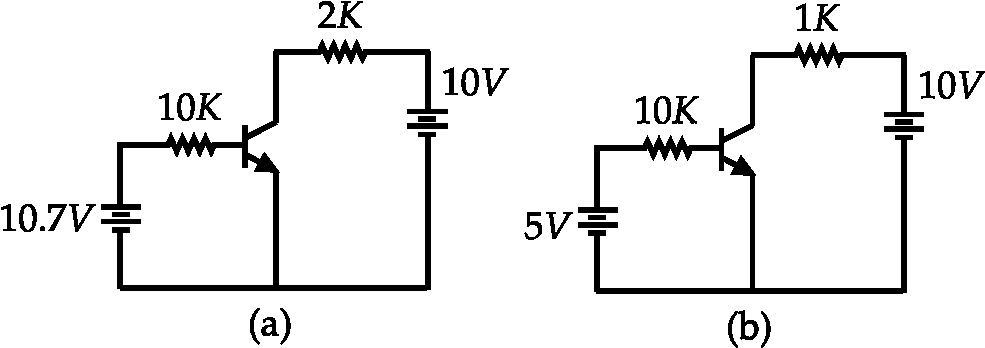
\includegraphics[height=3.2cm,width=9cm]{e-37}
	\end{figure}
	If the transistors in Figures (a) and (b) have current gain $\left(\beta_{d c}\right)$ of 100 and 10 respectively, then they operate in the
{	\exyear{NET/JRF(JUNE-2015)}}
\begin{tasks}(1)
\task[\textbf{A.}] Active region and saturation region respectively
\task[\textbf{B.}] Saturation region and active region respectively
\task[\textbf{C.}] Saturation region in both cases
\task[\textbf{D.}]  Active region in both cases
\end{tasks}
\begin{answer}
\begin{align*}
\intertext{In both case input section is F.B.}
\text{For figure (a) }I_{B}&=\frac{10.7-0.7}{10}=1 \mathrm{~mA} \Rightarrow I_{C}=B I_{B}=100 \mathrm{~mA}\\
\text{Thus }V_{C B}&=V_{C}-V_{B}=(10-2 \times 100)-0.7=-v e\\
&\Rightarrow \quad\text{ output section is F.B.}
\intertext{since both section are F.B. so it is in saturation region.}
\text{For Figure (b) }I_{B}&=\frac{5-0.7}{10}=0.43 \mathrm{~mA} \Rightarrow I_{C}=B I_{B}=4.3 \mathrm{~mA}\\
\text{Thus }V_{C B}&=V_{C}-V_{B}=(10-4.3)-0.7=+v e\\
&\Rightarrow \quad\text{ out put section is R.B.}
\intertext{Thus it is in active region}
\end{align*}
So the correct answer is \textbf{Option (B)}
\end{answer}
	\item The $I-V$ characteristics of a device can be expressed as $I=I_{s}\left[\exp \left(\frac{a V}{T}\right)-1\right]$, where $T$ is the temperature and $a$ and $I_{s}$ are constants independent of $T$ and $V$. Which one of the following plots is correct for a fixed applied voltage $V$ ?
{	\exyear{NET/JRF(DEC-2016)}}
\begin{tasks}(2)
\task[\textbf{A.}] \begin{figure}[H]
	\centering
	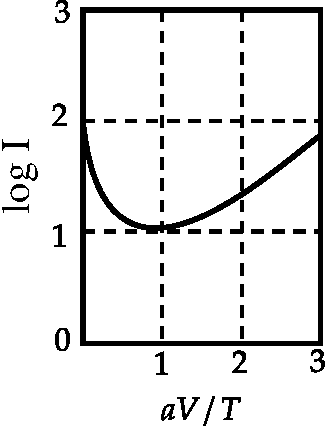
\includegraphics[height=4.5cm,width=3.5cm]{e48a}
\end{figure}
\task[\textbf{B.}] \begin{figure}[H]
	\centering
	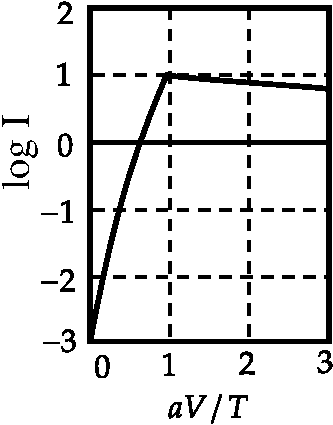
\includegraphics[height=4.5cm,width=3.5cm]{e48b}
\end{figure}
\task[\textbf{C.}] \begin{figure}[H]
	\centering
	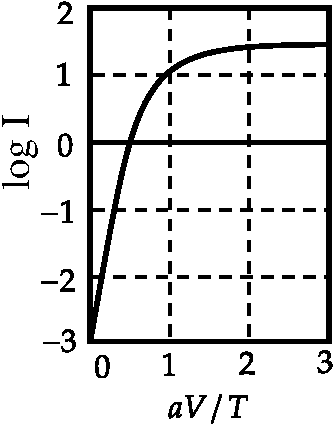
\includegraphics[height=4.5cm,width=3.5cm]{e48c}
\end{figure}
\task[\textbf{D.}] \begin{figure}[H]
	\centering
	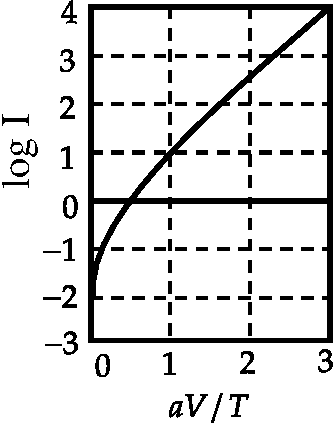
\includegraphics[height=4.5cm,width=3.5cm]{e48d}
\end{figure}
\end{tasks}
\begin{answer}
\begin{align*}
\text{Let }\frac{a v}{T}&=x\text{ For large }x ; \quad I=I_{s} e^{x} \Rightarrow \log _{e} I\\&=\log _{e} I s+x \Rightarrow \log _{e} I \propto x
\end{align*}
So the correct answer is \textbf{Option (D)}
\end{answer}
	\item In the $n$-channel JFET shown in figure below, $V_{i}=-2 V, C=10 p F, V_{D D}=+16 \mathrm{~V}$ and $R_{D}=2 k \Omega$\\
	\begin{figure}[H]
		\centering
		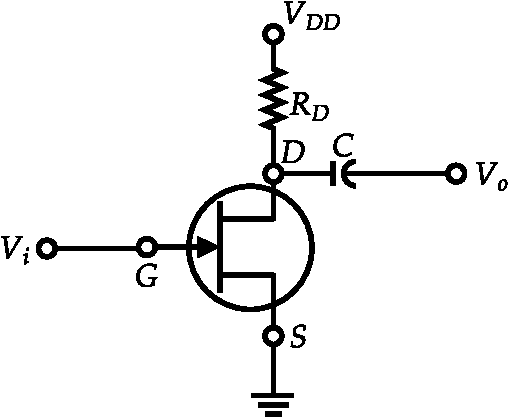
\includegraphics[height=4cm,width=5cm]{e53}
	\end{figure}
	If the drain $D$ - source $S$ saturation current $I_{D S S}$ is $10 m A$ and the pinch-off voltage $V_{P}$ is $-8 V$, then the voltage across points $D$ and $S$ is
{	\exyear{NET/JRF(JUNE-2017)}}
\begin{tasks}(4)
\task[\textbf{A.}] $11.125 \mathrm{~V}$
\task[\textbf{B.}] $10.375 \mathrm{~V}$
\task[\textbf{C.}] $5.75 \mathrm{~V}$
\task[\textbf{D.}] $4.75 \mathrm{~V}$
\end{tasks}
\begin{answer}
\begin{align*}
V_{G S Q}&=-V_{G G}=-2 V\\
I_{D Q}&=I_{D S S}\left(1-\frac{V_{G S}}{V_{P}}\right)^{2}=10 m A\left(1-\frac{-2}{-8}\right)^{2}=5.63 m A\\
V_{D S}&=V_{D D}-I_{D} R_{D}=16-5.63 \times z \approx 4.8 V
\end{align*}
So the correct answer is \textbf{Option (D)}
\end{answer}
	\item In the circuit below the voltages $V_{B B}$ and $V_{C C}$ are kept fixed, the voltage measured at $B$ is a constant, but that measured at $A$ fluctuates between a few $\mu V$ to a few $m V$.\\
	From these measurements it may be inferred that the
	{\exyear{NET/JRF(DEC-2017)}}
\begin{figure}[H]
\centering
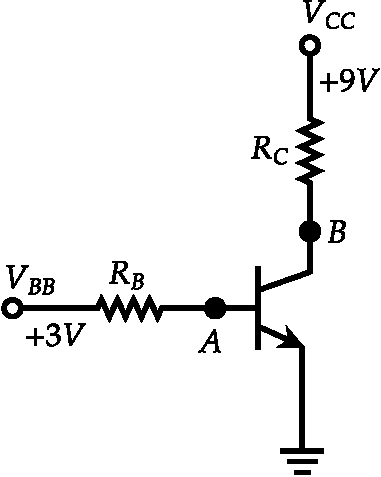
\includegraphics[height=4.5cm,width=4cm]{e63}
\end{figure}
\begin{tasks}(2)
\task[\textbf{A.}] Base is open internally
\task[\textbf{B.}] Emitter is open internally
\task[\textbf{C.}] Collector resistor is open
\task[\textbf{D.}] Base resistor is open
\end{tasks}
\begin{answer}
So the correct answer is \textbf{Option (D)}
\end{answer}
	\item In the following circuit, the value of the common-emitter forward current amplification factor $\beta$ for the transistor is 100 and $V_{B E}$ is $0.7 \mathrm{~V}$.\\
	\begin{figure}[H]
		\centering
		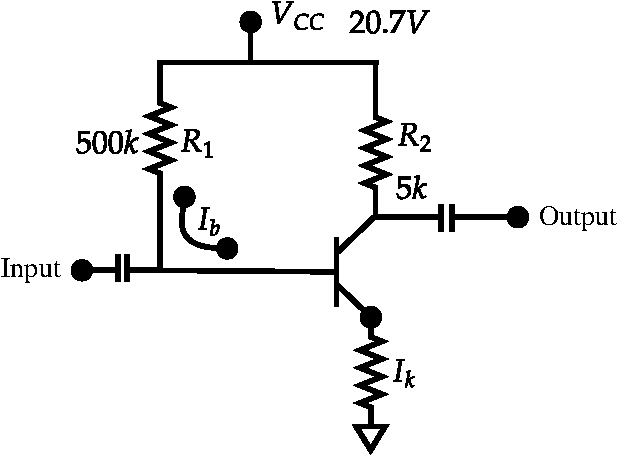
\includegraphics[height=4cm,width=5.5cm]{e68}
	\end{figure}
	The base current $I_{B}$ is
{	\exyear{NET/JRF(JUNE-2018)}}
\begin{tasks}(4)
\task[\textbf{A.}] $40 \mu A$
\task[\textbf{B.}] $30 \mu A$
\task[\textbf{C.}] $44 \mu A$
\task[\textbf{D.}] $33 \mu A$
\end{tasks}
\begin{answer}
\begin{align*}
I_{B}&=\frac{V_{c c}-V_{B E}}{R_{B}+\beta R_{E}}=\frac{20.7-0.7}{500+100 \times 1}\\&=\frac{20}{600 K}=\frac{20 \times 1000}{600} \mu A=33.3 \mu A
\end{align*}
So the correct answer is \textbf{Option (D)}
\end{answer}
	\item A sinusoidal signal is an input to the following circuit\\
	\begin{figure}[H]
		\centering
		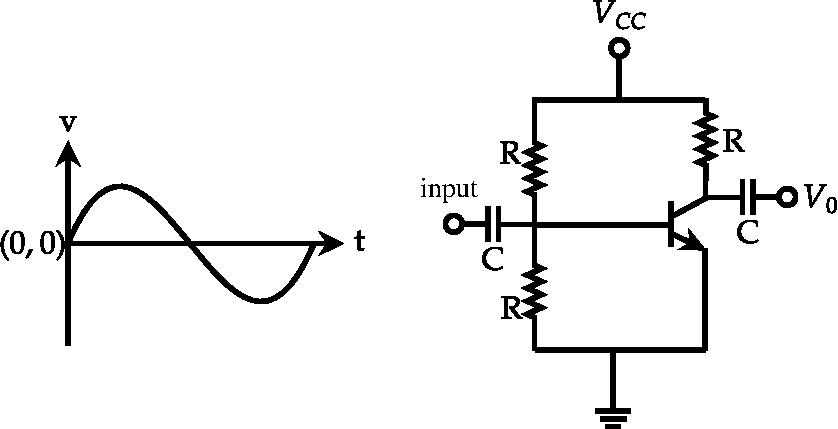
\includegraphics[height=5cm,width=8cm]{e75}
	\end{figure}
	Which of the following graphs best describes the output wave function?
{	\exyear{NET/JRF(DEC-2018)}}
\begin{tasks}(2)
\task[\textbf{A.}] \begin{figure}[H]
	\centering
	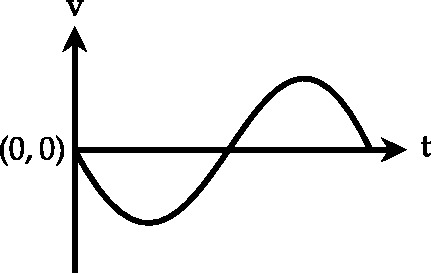
\includegraphics[height=3cm,width=5cm]{e75a}
\end{figure}
\task[\textbf{B.}] \begin{figure}[H]
	\centering
	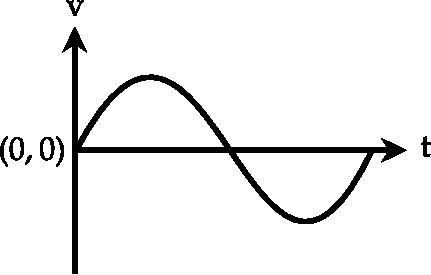
\includegraphics[height=3cm,width=5cm]{e75b}
\end{figure}
\task[\textbf{C.}] \begin{figure}[H]
	\centering
	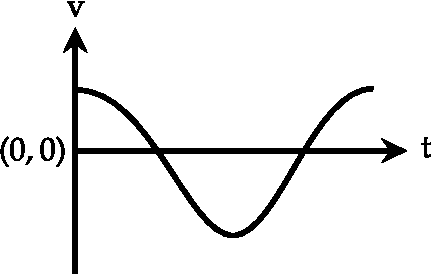
\includegraphics[height=3cm,width=5cm]{e75c}
\end{figure}
\task[\textbf{D.}] \begin{figure}[H]
	\centering
	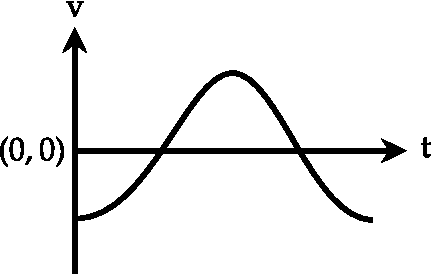
\includegraphics[height=3cm,width=5cm]{e76d}
\end{figure}
\end{tasks}
\begin{answer}
\begin{align*}
\text{In $CE$ transistor output has phase charge of $\pi$}
\end{align*}
So the correct answer is \textbf{Option (A)}
\end{answer}
	\item An $npn$ -transistor is connected in a voltage divider configuration as shown in the figure below\\
	\begin{figure}[H]
		\centering
		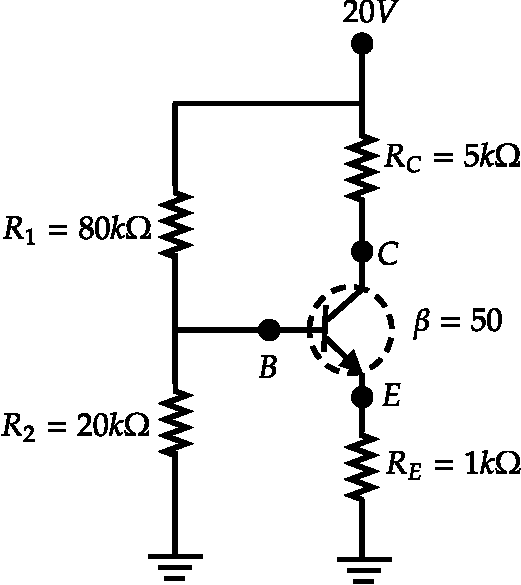
\includegraphics[height=6cm,width=5.5cm]{e-2}
	\end{figure}
	If the resistor $R_{2}$ is disconnected, the voltages $V_{B}$ at the base and $V_{C}$ at the collector change as follows.
{	\exyear{NET/JRF(JUNE-2019)}}
\begin{tasks}(2)
\task[\textbf{A.}]  Both $V_{B}$ and $V_{C}$ increase
\task[\textbf{B.}] Both $V_{B}$ and $V_{C}$ decrease
\task[\textbf{C.}]  $V_{B}$ decreases, but $V_{C}$ increases
\task[\textbf{D.}] $V_{B}$ increases, but $V_{C}$ decreases
\end{tasks}
\begin{answer}
\begin{align*}
V_{B}&=\frac{V_{C C} R_{2}}{R_{1}+R_{2}}=\frac{V_{C C}}{R_{1} / R_{2}+1} \quad\text{ as} R_{2} \uparrow, V_{B} \uparrow\\
\because V_{E}&=V_{B}-V_{B E}\text{ and }I_{E}=\frac{V_{E}}{R_{E}} \approx I_{C}\\
\text{As }&V_{B} \uparrow, V_{E} \uparrow\text{ thus }I_{E} \approx I_{C} \uparrow\\
\because V_{C C}&=V_{C C}-I_{C} R_{c}, \quad\text{ as }I_{C} \uparrow, V_{C} \downarrow
\end{align*}
So the correct answer is \textbf{Option (D)}
\end{answer}
	\item In a collector feedback circuit shown in the figure below, the base emitter voltage $V_{B E}=0.7 V$ and current gain $\beta=\frac{I_{C}}{I_{B}}=100$ for the transistor\\
	\begin{figure}[H]
		\centering
		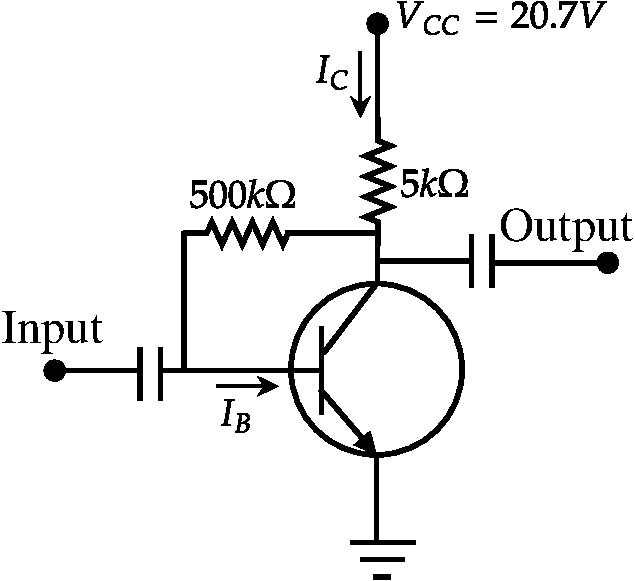
\includegraphics[height=5.5cm,width=6cm]{e-3}
	\end{figure}
	The value of the base current $I_{B}$ is
{	\exyear{NET/JRF(DEC-2019)}}
\begin{tasks}(4)
\task[\textbf{A.}] $20 \mu \mathrm{A}$
\task[\textbf{B.}]  $40 \mu \mathrm{A}$
\task[\textbf{C.}] $10 \mu \mathrm{A}$
\task[\textbf{D.}] $100 \mu \mathrm{A}$
\end{tasks}
\begin{answer}
\begin{align*}
\intertext{Apply K.V.L in input section}
-20 V+B I_{B} \times 5 K+I_{B} \times 500 K+0.7 V&=0\\
\Rightarrow I_{B}=\frac{193}{100 \times 5 K+500 K}&=19.3 \mu \mathrm{A}
\end{align*}
So the correct answer is \textbf{Option (A)}
\end{answer}
	
	
	
\end{enumerate}